\section{Implementation}

\subsection{Technical implementation}
\label{sec:technical}

The project is written in Python with pandas, scikit-learn and matplotlib (The pandas
development team 2024; scikit-learn developers 2025; The Matplotlib Development Team 2025); PyTorch is used only
for the two language models (Ansel et al.\ 2024). The \code{explorer} package has three layers (data and features,
model execution, explanation), with one module per pipeline step, all run through one command-line tool;
\code{config/settings.json} holds every threshold, window, grid and seed. Versions are pinned in a conda environment, and \V{tech.tests} tests check properties such as time
safety and the guardrail. A full rebuild runs offline, and a script compares the rebuilt tables with the committed
ones number by number (Pineau et al.\ 2021).

TxGPT was trained on GPUs in three sizes with three seeds each; the sizes tie, so the smallest
(\V{txgpt.s_params} parameters) was kept. The Assistant follows a modern decoder design (Touvron et al.\ 2023) and was
pretrained on \V{lm.pretrain_tokens} billion DS5 tokens, more than the compute-optimal budget of about 20 tokens per
parameter (Hoffmann et al.\ 2022), then taught conversation (DS6) and explanations (DS7). It predicts on a CPU.

The \code{Predictor} class is the interface Assignment~3 will call. Three commands expose it: \code{predict address}
scores an address's whole timeline, \code{predict what-if} scores a hypothetical next transaction (the brief's
``user input to prediction''), and \code{predict explain} explains any transaction.

\subsection{Implementation evaluation}
\label{sec:evaluation}

\textbf{Objectives.} Table~\ref{tab:objectives} compares the results with Assignment~1's targets. The baseline meets the recall target on spikes and dormant addresses but not on bursts counted per
transaction (\V{ds1.baseline.burst_tx}), although it finds \V{ds1.baseline.burst_event} of burst events, and four
DS1 addresses break the sanity rule. We report these rather than move the targets. Two objectives that need people
outside the build remain open.

\begin{table}[htbp]
\centering
\footnotesize
\caption{Assignment~1's objectives for the selected method (the robust z baseline) and the results.}
\label{tab:objectives}
\begin{tabularx}{\textwidth}{@{}Y L{5.6cm} l@{}}
\toprule
Objective (set in Assignment~1) & Result & Status \\
\midrule
Snapshot of 20--30 main addresses (50+ tx, 90+ days) and 2--3 short ones & 25 main and 3 short addresses & Met \\
Planted recall $\geq$ 70\% for 2 of 3 patterns & Spike 0.744, dormant 0.840, burst 0.381 & Met \\
Stability: top-50 Jaccard $\geq$ 0.7 & 1.000 & Met \\
Sanity: no address over 20\% flagged & DS1: 4 addresses over; DS10: 0 & Partly met \\
Method agreement reported & Baseline--fusion Jaccard 0.512 & Met \\
Blind reviewer check (Cohen's kappa) & Pending: two teammates rate reports/reviewer/sheet.csv & Open \\
Accuracy, precision, recall, F1 where labels exist & DS3 and DS4 (Table~\ref{tab:classifiers}) & Met \\
\bottomrule
\end{tabularx}
\end{table}


\textbf{Scoring methods on DS1} (Table~\ref{tab:ds1}). Each method finds different patterns
(Figure~\ref{fig:recall}). Regression finds every planted burst event but few dormant addresses, LOF misses most
spikes, and only fusion, the baseline and TxGPT catch most spikes, burst events and dormant addresses. TxGPT flags
the fewest real transactions (\V{ds1.txgpt.flag_rate}) and so has the highest precision lower bound
(\V{ds1.txgpt.precision} against \V{ds1.baseline.precision}); a flag that is not a plant may still be worth a look,
so real-data precision can only be bounded.

\begin{table}[htbp]
\centering
\footnotesize
\caption{Scoring methods on DS1 (sorted by mean planted recall).}
\label{tab:ds1}
\begin{tabularx}{\textwidth}{@{}L{3.6cm} l r r r l r R@{}}
\toprule
Method & Family & Spike & Burst & Dormant & Mean [95\% CI] & Stab. & Flags \\
\midrule
Score fusion & Combination & 0.780 & 0.498 & 0.768 & 0.682 [0.573, 0.781] & 0.736 & 9.4\% \\
Robust z baseline (A1) $\star$ & Statistics & 0.744 & 0.381 & 0.840 & 0.655 [0.546, 0.753] & 1.000 & 10.4\% \\
Regression residual & Regression & 0.864 & 0.695 & 0.320 & 0.626 [0.526, 0.722] & 0.736 & 17.5\% \\
TxGPT surprisal & Sequence model & 0.736 & 0.170 & 0.736 & 0.547 [0.442, 0.638] & 1.000 & 1.5\% \\
DBSCAN distance & Clustering & 0.544 & 0.109 & 0.776 & 0.476 [0.366, 0.571] & 0.912 & 3.9\% \\
K-Means distance & Clustering & 0.624 & 0.050 & 0.736 & 0.470 [0.359, 0.567] & 1.000 & 3.8\% \\
Isolation Forest & Outlier detection & 0.600 & 0.122 & 0.564 & 0.429 [0.321, 0.534] & 0.876 & 3.6\% \\
Local Outlier Factor & Outlier detection & 0.116 & 0.066 & 0.812 & 0.331 [0.262, 0.392] & 0.846 & 4.5\% \\
Regression range (conformal) & Regression & 0.712 & 0.174 & 0.044 & 0.310 [0.246, 0.373] & 0.514 & 4.8\% \\
\bottomrule
\end{tabularx}
\par\smallskip\parbox{\textwidth}{\footnotesize Recall on planted transactions over five reporting seeds; intervals are 95\% address-level bootstrap. Burst is per transaction; mean recall averages spike, burst and dormant. Stability is the top-50 Jaccard over refits. Flag rate is the share of real evaluation-period transactions flagged. $\star$ the selected method.}
\end{table}


\begin{figure}[ht]
\centering
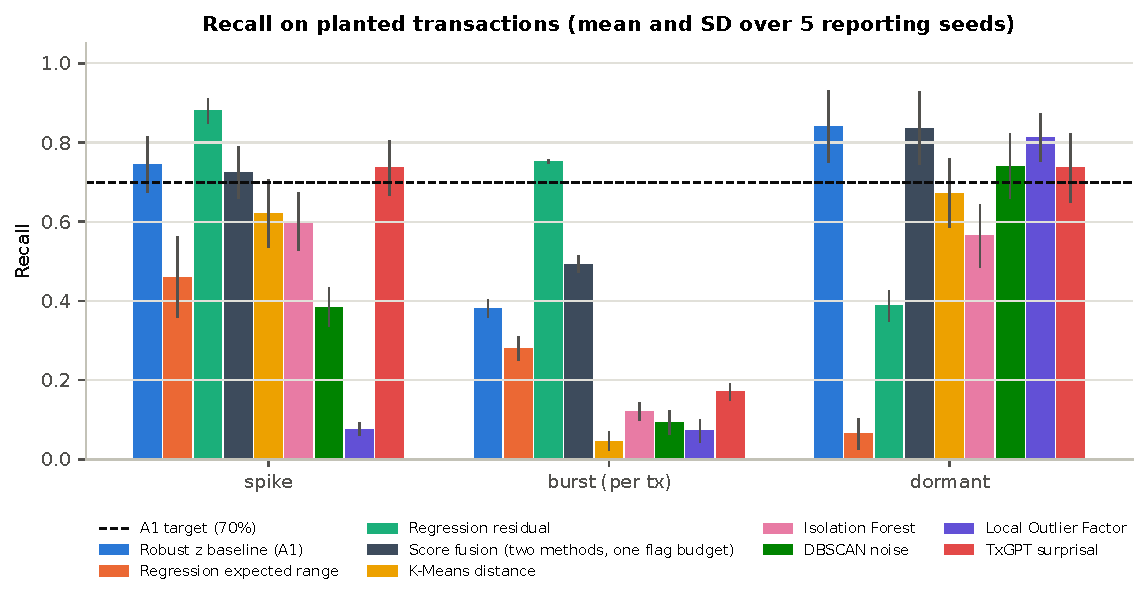
\includegraphics[width=0.8\textwidth]{eval_injection_recall.pdf}
\caption{Recall on planted transactions by pattern (mean and standard deviation over five reporting seeds). No
method is best at every pattern; the dashed line is Assignment~1's 70\% target.}
\label{fig:recall}
\end{figure}

\textbf{Regression and clustering} (Table~\ref{tab:unsupervised}). The random forest cuts the naive forecast's
error by \V{reg.gap_skill} on gaps but only \V{reg.size_skill} on amounts. Conformal calibration lifts the amount
range's coverage from \V{conf.before} to \V{conf.after} against a nominal \V{conf.nominal}, still slightly short.

\begin{table}[htbp]
\centering
\footnotesize
\caption{Regression and clustering metrics on DS1.}
\label{tab:unsupervised}
\begin{tabularx}{\textwidth}{@{}l Y r r r r@{}}
\toprule
Target & Model & MAE & RMSE & $R^2$ & Skill \\
\midrule
Amount & Naive forecast & 0.186 & 0.416 & 0.730 & 0.000 \\
Amount & Ridge & 0.181 & 0.373 & 0.783 & 0.027 \\
Amount & Random forest & 0.168 & 0.368 & 0.788 & 0.099 \\
Amount & Hist.\ gradient boosting & 0.189 & 0.389 & 0.764 & $-$0.015 \\
Gap & Naive forecast & 0.476 & 0.665 & 0.039 & 0.000 \\
Gap & Ridge & 0.279 & 0.410 & 0.635 & 0.414 \\
Gap & Random forest & 0.189 & 0.301 & 0.803 & 0.603 \\
Gap & Hist.\ gradient boosting & 0.192 & 0.298 & 0.807 & 0.597 \\
\bottomrule
\end{tabularx}
\par\smallskip\parbox{\textwidth}{\footnotesize Regression on the evaluation period, log10 scale; skill is 1 $-$ MAE / the naive forecast's MAE. Clustering, first search before the stages: K-Means $k=2$, silhouette 0.657, Davies--Bouldin 0.834; DBSCAN radius 1.3$\times$ the k-distance elbow, silhouette 0.786 without noise points, 2.0\% noise.}
\end{table}


\textbf{Agreement and stability over time.} The methods flag different transactions: the baseline's overlap
(Jaccard) with the other single methods is only \V{agree.base_range}, and \V{agree.base_txgpt} with TxGPT. Refitting
at \V{wf.cutoffs} walk-forward cut-offs keeps the baseline's mean recall at \V{wf.baseline_range}, so its result
does not depend on one split; LOF varies more (\V{wf.lof_range}).

\textbf{Unseen addresses: DS2 and DS10.} The frozen methods were tested on \V{ds2.check_addresses} DS2
histories and once on DS10 (Figure~\ref{fig:ds10}). Two outcomes were unexpected. First, methods tuned on DS1 fall
the most: fusion drops from \V{ds1.fusion.mean} to \V{ds10.fusion.mean} on DS10, below the baseline's
\V{ds10.baseline.mean}. Second, TxGPT, which learned from other addresses, ranks first on DS10
(\V{ds10.txgpt.mean}, interval \V{ds10.txgpt.ci}). Over 100 plant seeds the baseline ranks first among the
pooled methods on DS10 in \V{stats.ds10_baseline_rank1} of seeds. Bursts are hard to find on DS10, whose addresses
are busier and less regular (median gap \V{act.ds10_gap} hours against \V{act.ds1_gap} on DS1).

\begin{figure}[ht]
\centering
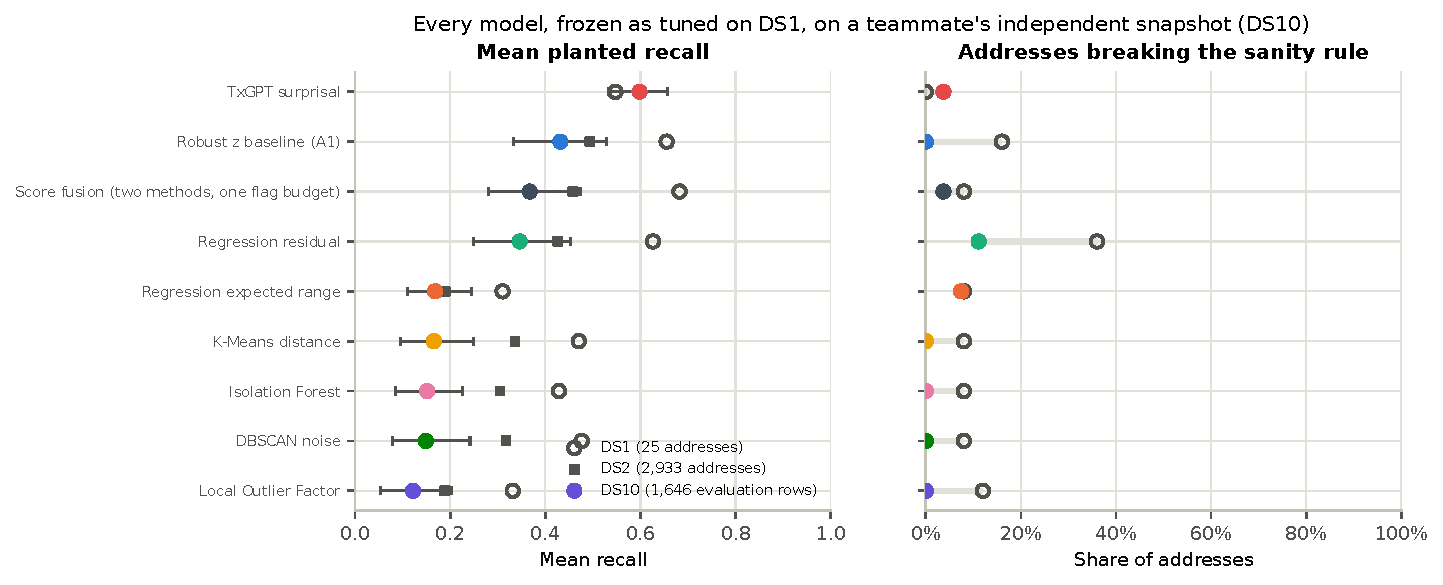
\includegraphics[width=0.95\textwidth]{eval_ds10_check.pdf}
\caption{Every method, frozen as tuned on DS1, on DS2 and the held-out DS10 (left: mean planted recall with
95\% bootstrap intervals on DS10; right: share of addresses breaking the sanity rule).}
\label{fig:ds10}
\end{figure}

\textbf{Classifiers on labelled data} (Table~\ref{tab:classifiers}). On Elliptic the random forest has the best
F1 (\V{cls.ell_rf_f1}, interval \V{cls.ell_rf_f1_ci} over ten training seeds), but every model collapses from
time step 43 (Figure~\ref{fig:elliptic}, Appendix~\ref{app:figures}), when a dark market closed and illicit behaviour changed (Pareja et al.\
2020). On BitcoinHeist's temporal split no model's F1 exceeds \V{cls.heist_temporal_max_f1}, and families held out of
training are found at recalls of \V{cls.lofo_range} by the tree models, consistent with Finding~4.

\begin{table}[htbp]
\centering
\footnotesize
\caption{Classifiers on the labelled datasets.}
\label{tab:classifiers}
\begin{tabularx}{\textwidth}{@{}L{3.6cm} Y r r r r r@{}}
\toprule
Data and split & Model & Accuracy & Precision & Recall & F1 & PR-AUC \\
\midrule
Elliptic, all features & Hist.\ gradient boosting & 0.971 & 0.808 & 0.734 & 0.769 & 0.803 \\
Elliptic, all features & k-nearest neighbours & 0.957 & 0.684 & 0.620 & 0.650 & 0.659 \\
Elliptic, all features & Logistic regression & 0.949 & 0.619 & 0.578 & 0.598 & 0.412 \\
Elliptic, all features & Random forest & 0.979 & 0.928 & 0.727 & 0.815 & 0.792 \\
Elliptic, local features & Hist.\ gradient boosting & 0.965 & 0.738 & 0.721 & 0.730 & 0.784 \\
Elliptic, local features & k-nearest neighbours & 0.969 & 0.792 & 0.703 & 0.745 & 0.741 \\
Elliptic, local features & Logistic regression & 0.969 & 0.839 & 0.640 & 0.726 & 0.619 \\
Elliptic, local features & Random forest & 0.970 & 0.801 & 0.721 & 0.759 & 0.781 \\
BitcoinHeist, temporal & Hist.\ gradient boosting & 0.705 & 0.012 & 0.722 & 0.024 & 0.042 \\
BitcoinHeist, temporal & k-nearest neighbours & 0.789 & 0.011 & 0.452 & 0.021 & 0.025 \\
BitcoinHeist, temporal & Logistic regression & 0.170 & 0.006 & 0.976 & 0.012 & 0.005 \\
BitcoinHeist, temporal & Random forest & 0.942 & 0.038 & 0.436 & 0.070 & 0.052 \\
BitcoinHeist, random & Hist.\ gradient boosting & 0.975 & 0.199 & 0.252 & 0.222 & 0.151 \\
BitcoinHeist, random & k-nearest neighbours & 0.957 & 0.099 & 0.254 & 0.143 & 0.071 \\
BitcoinHeist, random & Logistic regression & 0.510 & 0.020 & 0.691 & 0.039 & 0.017 \\
BitcoinHeist, random & Random forest & 0.979 & 0.250 & 0.239 & 0.244 & 0.177 \\
\bottomrule
\end{tabularx}
\par\smallskip\parbox{\textwidth}{\footnotesize Test splits: Elliptic time steps 35--49; BitcoinHeist years after the training years (temporal) or a random 20\%. Metrics are for the datasets' own positive classes (illicit; ransomware), at the threshold chosen on validation data.}
\end{table}


\textbf{Unusual is not a label.} Scored against the labelled classes, the unsupervised methods do worse than chance
(PR-AUC below the class share), while the random forest reaches \V{label.ell_rf_lift}$\times$ chance on Elliptic
(Appendix~\ref{app:figures}). Being unusual and belonging to a labelled class are different things, which supports
the Explorer's wording.

\textbf{Language models.} The Assistant passes the guardrail on \V{lm.guard_ds7} of DS7 test prompts and
\V{lm.guard_ds10} of DS10 prompts, and is fully correct (right reasons, order and numbers) on \V{lm.full_ds7} and
\V{lm.full_ds10}; pooled over twelve test sets, \V{lm.pooled} (\V{lm.pooled_ci}). Its weakest area is open glossary
questions, where it states \V{lm.glossary} of the key facts.

\textbf{Limitations.} Plants are our guess at what unusual looks like; DS1 has only 28 addresses, so intervals are
wide; methods tuned on DS1 transfer less well; and a language model can still give a wrong reason the guardrail
misses, so the template remains the default.
